\chapter{Implementazione del ChatBot}
\label{cap:chatbot}

Per completare l'apprendimento dei token \emph{JWT} e dei vari metodi di autenticazione, è stato richiesto di implementare un \emph{ChatBot} per la piattaforma Microsoft Teams che si interfacciasse con i servizi \emph{API} dell'azienda.
L'intero codice è stato scritto in \emph{C\#} e utilizzando il framework \emph{.NET Core 8.0}.

\bigskip

\begin{figure}[!ht]
    \centering
    \begin{minipage}[t]{0.5\textwidth}
        \centering
        
\includegraphics[width=0.25\textwidth]{chatbot/csharp-icon}
        \caption{Logo di C\#}
    \end{minipage}\hfill
    \begin{minipage}[t]{0.5\textwidth}
        \centering
        
\includegraphics[width=0.25\textwidth]{chatbot/dotnet-icon}
        \caption{Logo di .NET Core}
    \end{minipage}
\end{figure}

\section{Architettura}

Il \emph{ChatBot} si compone di due parti principali: il \emph{Bot} vero e proprio e il l'\emph{HttpListener} (o \emph{WebServer}). 
Il primo è responsabile dell'autenticazione del \emph{Bot} e della gestione delle \emph{chat} con gli utenti, mentre il secondo si occupa della ricezione delle notifiche tramite \emph{HTTP}.

Il \emph{Bot} è in grado di creare nuove conversazioni, inviare nuovi messaggi e creare \emph{subscription}.

Una \emph{subscription} è un meccanismo che permette di ricevere notifiche in tempo reale da un servizio \emph{API}, in questo caso da Microsoft Teams attraverso il servizio \emph{Graph API}.
Per creare una \emph{subscription} è necessario specificare l'\emph{endpoint}\footnote{Un endpoint è un URL che rappresenta una specifica risorsa o funzionalità in un'API. Gli endpoint consentono ai client di interagire con i server tramite HTTP(S)} a cui inviare le notifiche, il tipo di evento da monitorare e il \emph{certificato} per la cifratura delle notifiche.

L'\emph{HttpListener}, invece, si occupa della gestione delle notifiche generate dalle \emph{subscription}, validando i dati ricevuti e inviando le risposte al \emph{Bot}.

Entrambe la parti, dunque, si interfacciano con il servizio \emph{Graph API} che funziona da \emph{proxy}\footnote{un proxy è un server intermedio che si interpone tra il client e il server per filtrare le richieste, migliorare le prestazioni e garantire la sicurezza delle comunicazioni.} per le richieste verso Microsoft Teams.

L'\emph{HttpListener} inoltre è stato predisposto per comunicare con le API dell'azienda, che hanno il compito di elaborare i dati decrittografati e, tramite l'utilizzo di \emph{Intelligenza Artificiale}, generare una risposta.
Questa risposta viene poi inoltrata al \emph{Bot} che la invia all'utente (figura \ref{fig:arch-bot}).

\begin{figure}[!ht] 
    \centering 
    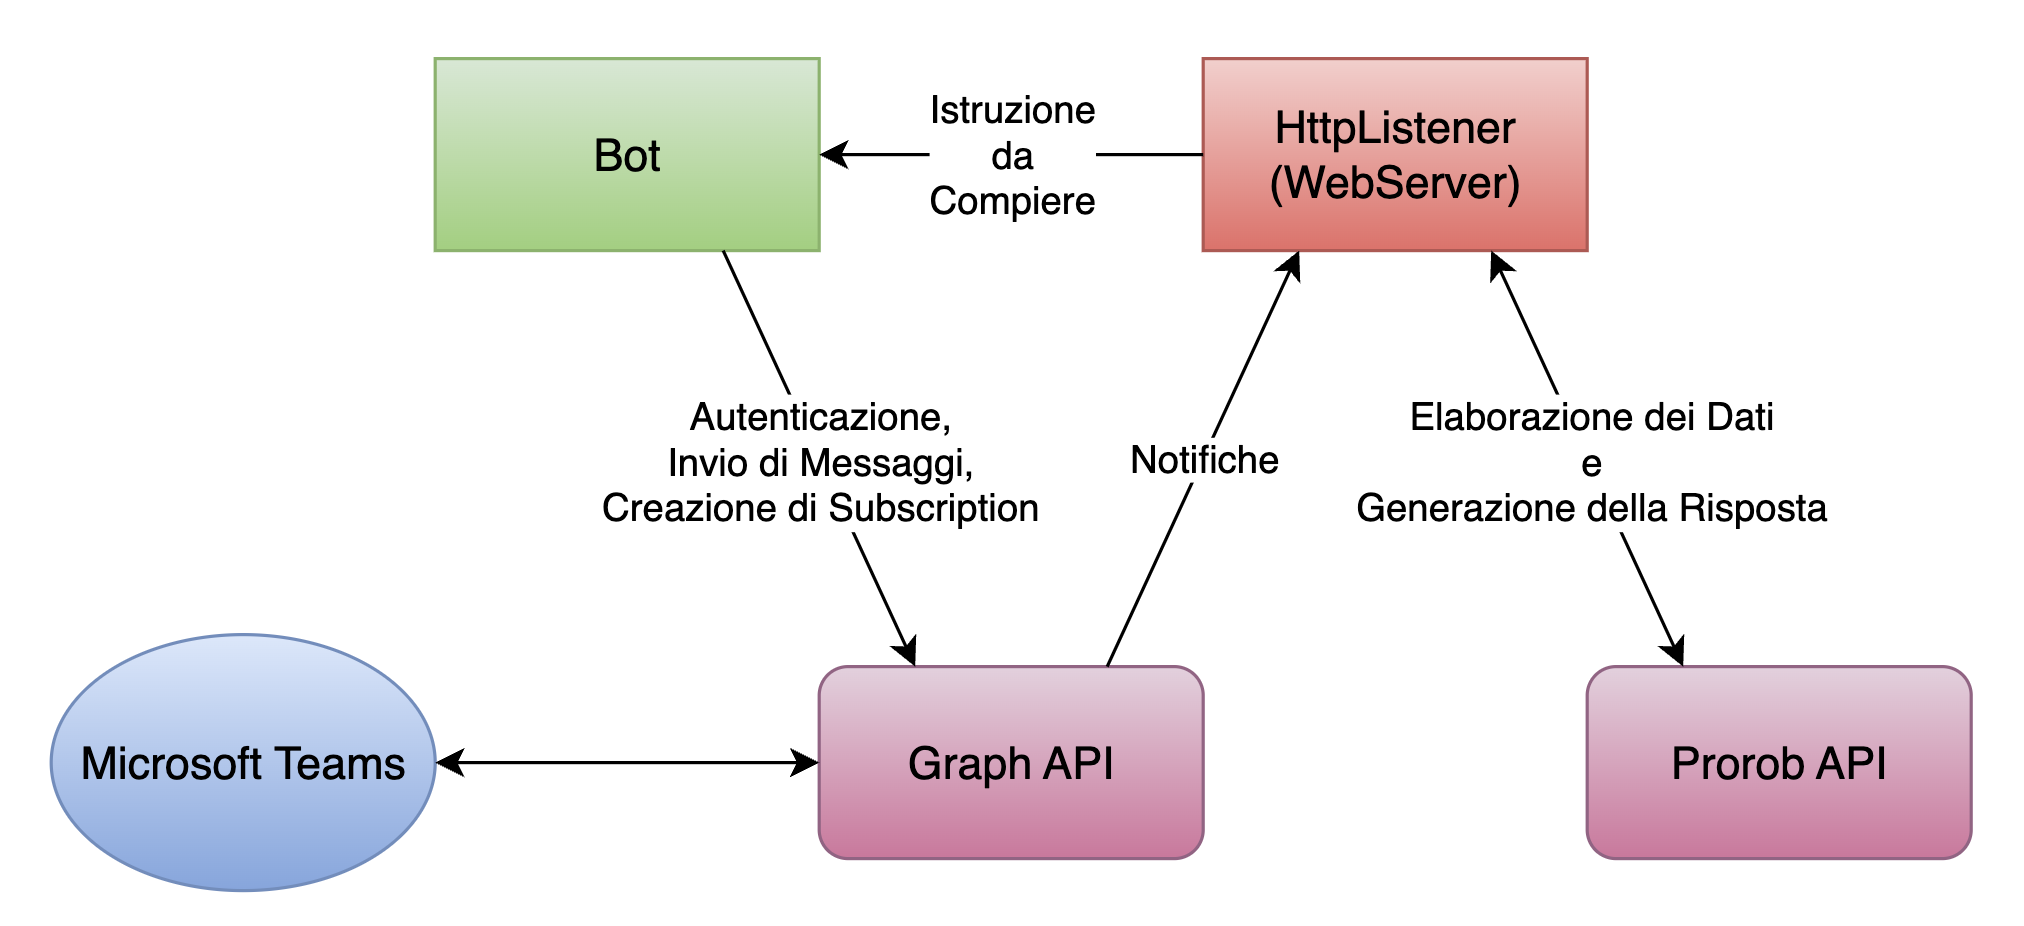
\includegraphics[width=1\columnwidth]{chatbot/architettura} 
    \caption{Architettura del ChatBot}
	\label{fig:arch-bot}
\end{figure}

\section{Utilizzo di token e crittografia}

I token \emph{JWT} sono stati utilizzati in due casi per il funzionamento del \emph{ChatBot}:
\begin{itemize}
	\item Per l'autenticazione del \emph{Bot} con il servizio \emph{Graph API} di Microsoft.
	\item Per la verifica dell'autenticità delle notifiche inviate dal servizio \emph{Graph API} al \emph{WebServer}.
\end{itemize}

Il primo caso viene gestito automaticamente dalla libreria \emph{Microsoft.Graph} che si occupa di generare e rinnovare i token necessari per l'autenticazione.
Questo processo è trasparente all'utente e non richiede alcuna configurazione aggiuntiva.

Il secondo caso, invece, è gestito manualmente, verificando la firma del token ricevuto dal servizio \emph{Graph API}.
Inoltre, il contenuto delle notifiche viene crittografato con un \emph{certificato \gls{X.509}} per garantire la riservatezza delle informazioni.

\subsection{Creazione dei certificati}

\noindent La creazione dei \emph{certificati} avviene tramite il codice mostrato nel listing \ref{lst:rsa-code}.

\definecolor{darkgreen}{rgb}{0.0, 0.5, 0.0}

\lstset{
    language=[Sharp]C,
    basicstyle=\ttfamily,
    keywordstyle=\color{blue},
    stringstyle=\color{red},
    commentstyle=\color{darkgreen},
    tabsize=4,
    numbers=left,
    numberstyle=\color{gray},
    breaklines=true,
    captionpos=b,
    frame=single,
    showspaces=false,
    showstringspaces=false,
    breakatwhitespace=true,
    columns=fullflexible,
}

\begin{lstlisting}[caption=Codice per la creazione di certificati tramite RSA, label=lst:rsa-code]
using RSA rsa = RSA.Create(2048);

CertificateRequest request =
	new(
		"cn=NotificationServiceCertificate",
		rsa,
		HashAlgorithmName.SHA256,
		RSASignaturePadding.Pkcs1
	);

using X509Certificate2 cert = request.CreateSelfSigned(
	DateTimeOffset.Now,
	DateTimeOffset.Now.AddYears(5)
);

string certificateBase64String = Convert.ToBase64String(
	cert.Export(X509ContentType.Cert)
);

CertificateConfig newCertificate =
	new()
	{
		CERTIFICATE_ID = Certificates.GetUniqueId(),
		CERTIFICATE = certificateBase64String,
		PRIVATE_KEY = Convert.ToBase64String(rsa.ExportRSAPrivateKey())
	};
\end{lstlisting}

\bigskip

Si può notare che i certificati vengono creati da \emph{RSA} a 2048 bit e vengono firmati con l'algoritmo \emph{SHA-256} utilizzando il \emph{padding}\footnote{Il padding è una parte aggiuntiva al messaggio che consente di raggiungere la corretta lunghezza per l'algoritmo crittografico utilizzato.} dello standard \emph{PKCS\#1} (\emph{RS256}).
Siccome il \emph{certificato} include solo la chiave pubblica, è possibile utilizzare la chiave privata per creare una firma digitale da includere nel certificato. Naturalmente, questa firma potrà essere verificata da chiunque riceva il \emph{certificato}.

Il \emph{certificato} viene quindi convertito a stringa \emph{Base64} e salvato localmente con la chiave privata e un identificativo univoco.
Infine, viene inviato al servizio \emph{Graph API} per la creazione della \emph{subscription}, in modo che ogni sua notifica venga crittografata.

\subsection{Validazione delle notifiche}

Ogni notifica ricevuta deve essere validata seguendo certi passaggi che garantiscono l'autenticità del mittente e la riservatezza delle informazioni.

\noindent Il primo passo è la validazione dei token \emph{JWT}. 
\begin{enumerate}
	\item Il token non deve essere scaduto.
	\item È necessario, poi, verificare che il token non sia stato manomesso e che sia stato rilasciato da Microsoft ottenendo la chiave pubblica dall'\emph{endpoint} specificato nella documentazione\footcite{site:rich-notification}.
	\item Infine, è necessario verificare che il token sia stato rilasciato per la propria applicazione verificando che il campo \emph{audience} del token sia uguale all'\emph{AppId} dell'applicazione.
\end{enumerate}

\noindent La libreria \emph{Microsoft.IdentityModel.Tokens} ha fornito un aiuto per la validazione dei token, illustrata nel listing \ref{lst:jwt-verification-code}.

\begin{lstlisting}[caption=Codice per la verifica della firma nei token JWT, label=lst:jwt-verification-code]
private static async Task<bool> ValidateJwtToken(string token, IEnumerable<string> appIds)
{
	ConfigurationManager<OpenIdConnectConfiguration> configurationManager =
		new(
			"https://login.microsoftonline.com/common/v2.0/.well-known/
			openid-configuration",
			new OpenIdConnectConfigurationRetriever()
		);

	OpenIdConnectConfiguration openIdConfig =
		await configurationManager.GetConfigurationAsync();
	JwtSecurityTokenHandler handler = new();

	try
	{
		handler.ValidateToken(
			token,
			new TokenValidationParameters
			{
				ValidateIssuer = true,
				ValidateAudience = true,
				ValidateIssuerSigningKey = true,
				ValidateLifetime = true,
				ValidIssuer =
					$"https://login.microsoftonline.com/
					{ConfigManager.ConfigManager.Config.TENANT_ID}/v2.0",
				ValidAudiences = appIds,
				IssuerSigningKeys = openIdConfig.SigningKeys
			},
			out _
		);

		return true;
	}
	catch (Exception ex)
	{
		Logger.Logger.LogError(ex, "Error validating JWT token");
	}

	return false;
}
\end{lstlisting}

\bigskip

Una volta che è stata verificata la validità del token, si può procedere a decrittografare il contenuto della notifica.
Per questioni di efficienza, Microsoft Graph utilizza un processo di cifratura a due passaggi: viene infatti generata una chiave simmetrica per la cifratura del contenuto, mentre la chiave pubblica fornita dal \emph{certificato} viene utilizzata per cifrare la chiave simmetrica.

Questo processo permette di velocizzare la cifratura e la decifratura del contenuto, in quanto la cifratura asimmetrica è molto più lenta rispetto a quella simmetrica.

\noindent Si procede, dunque, come segue:
\begin{enumerate}
	\item Si utilizza la chiave privata per decrittografare il campo \emph{dataKey} del \emph{JSON} ottenuto dalla notifica utilizzando \emph{\gls{OAEP}} come \emph{padding}. Questo campo contiene la chiave simmetrica crittografata con la chiave pubblica.
	\item Prima di decrittografare il contenuto vero e proprio della notifica, la chiave simmetrica deve essere utilizzata per verificare la firma nel campo \emph{dataSignature}.
	Viene quindi calcolata la firma del campo \emph{data} e confrontata con il campo \emph{dataSignature}.
	\item A questo punto, solamente se la firma è valida, si può procedere con la decifratura del campo \emph{data} utilizzando la chiave simmetrica.
	Per questo passaggio si utilizza l'algoritmo \emph{AES} con \emph{padding PKCS\#7} e modalità di cifratura \emph{\gls{CBC}}. Come vettore di inizializzazione vengono utilizzati i primi 16 bytes della chiave simmetrica. 
	\item Il contenuto decrittografato risultante è un \emph{JSON} contenente le informazioni della notifica.
\end{enumerate}

\noindent Le funzioni sviluppate per eseguire queste operazioni sono state tre. La prima si occupa di decrittografare la chiave simmetrica con \emph{RSA}, la seconda di verificare la firma e la terza di decrittografare il contenuto con \emph{AES}.
Queste funzioni sono illustrate nel listing \ref{lst:decryption-code}.

\begin{lstlisting}[caption=Funzioni per la decifratura delle notifiche, label=lst:decryption-code]
// Decrypt the simmetric key with RSA
private static byte[] DecryptDataRsa(string privateKey, string encryptedData)
{
	using RSA rsa = RSA.Create(2048);

	rsa.ImportRSAPrivateKey(Convert.FromBase64String(privateKey), out _);

	byte[] encryptedDataBytes = Convert.FromBase64String(encryptedData);

	return rsa.Decrypt(encryptedDataBytes, RSAEncryptionPadding.OaepSHA1);
}


// Verify the signature
private static bool VerifySignature(byte[] key, string payload, string expectedSignature)
{
	byte[] payloadBytes = Convert.FromBase64String(payload);
	byte[] expectedSignatureBytes = Convert.FromBase64String(expectedSignature);
	byte[] actualSignature;

	using HMACSHA256 hmac = new(key);
	actualSignature = hmac.ComputeHash(payloadBytes);

	if (!actualSignature.SequenceEqual(expectedSignatureBytes))
	{
		return false;
	}

	return true;
}


// Decrypt the data with AES
private static byte[] DecryptDataAes(byte[] symmetricKey, string encryptedData)
{
	byte[] encryptedDataBytes = Convert.FromBase64String(encryptedData);

	int vectorSize = 16;
	byte[] iv = new byte[vectorSize];
	Array.Copy(symmetricKey, iv, vectorSize);

	using Aes aes = Aes.Create();
	aes.Key = symmetricKey;
	aes.IV = iv;

	using MemoryStream ms = new(encryptedDataBytes);
	using CryptoStream cs = new(ms, aes.CreateDecryptor(), CryptoStreamMode.Read);
	using MemoryStream output = new();

	cs.CopyTo(output);

	return output.ToArray();
}
\end{lstlisting}

\bigskip

\subsection{Gestione della sicurezza}

Come si può notare dalla sezione precedente, il processo di validazione delle notifiche è molto complesso e richiede l'utilizzo di algoritmi crittografici avanzati.
Questo è dovuto alla necessità di garantire sicurezza e riservatezza delle informazioni scambiate, mantenendo un alto livello di efficienza.
Infatti l'utilizzo di cifratura a due passaggi rende il processo molto più snello rispetto a una cifratura asimmetrica completa.
Inoltre, tutte le trasmissioni tra il \emph{WebServer} e le \emph{API} sono crittografate con il protocollo \emph{HTTPS}, aggiungendo un ulteriore livello di protezione.

Un altro aspetto da considerare è la gestione dei \emph{certificati}.
Questi vengono generati automaticamente e salvati in una struttura dati a dizionario\footnote{Il è una struttura dati che associa chiavi univoche a valori corrispondenti, permettendo accesso rapido ai valori tramite le loro chiavi.} che permette di recuperarli in modo efficiente.
È molto importante che le chiavi salvate in esso vengano fatte ruotare periodicamente per mitigare il rischio di compromissione.


\section{Gestione delle conversazioni}

Il \emph{WebServer} è stato implementato in modo da poter inviare il contenuto di una notifica alle \emph{API} dell'azienda dopo che è stato decrittografato.
Quando l'\emph{API} genera una risposta, questa viene riinviata al \emph{WebServer} che la inoltra al \emph{Bot} per l'invio all'utente.

Essendo l'ID della chat contenuto nella notifica, il \emph{Bot} è in grado di inviare la risposta alla conversazione corretta, con la possibilità di inviare, oltre al testo, anche immagini.

\noindent La funzione chiamata è \emph{SendChatMessage} ed è illustrata nel listing \ref{lst:send-message-code}.

\begin{lstlisting}[caption=Funzione per l'invio dei messaggi, label=lst:send-message-code]
public async Task<ChatMessage?> SendChatMessage(
	string chatId,
	string message,
	string? imagePath = null
)
{
	ChatMessage? requestBody;

	if (imagePath != null)
	{
		string extension = Path.GetExtension(imagePath);

		byte[]? imageBytes = null;

		int width = 314;
		int height = 314;

		try
		{
			imageBytes = File.ReadAllBytes(imagePath);

			using ImageSharp.Image<Rgba32> image = ImageSharp.Image.Load<Rgba32>(imagePath);

			width = image.Width;
			height = image.Height;
		}
		catch (Exception e)
		{
			Logger.Logger.LogError(e, "Error while reading the image");
		}

		double resizedHeight = (int)(314 * (double)height / width);
		width = 314;

		requestBody = new ChatMessage
		{
			Body = new ItemBody
			{
				ContentType = BodyType.Html,
				Content =
					"<div><span>"
					+ message
					+ "</span><img src=\"../hostedContents/1/$value\" style=\"vertical-align:bottom; width:"
					+ width
					+ "px; height:"
					+ resizedHeight
					+ "px\"></div>",
			},
			HostedContents =
			[
				new()
				{
					ContentBytes = imageBytes,
					ContentType = "image/png",
					AdditionalData = new Dictionary<string, object>
					{
						{ "@microsoft.graph.temporaryId", "1" },
					},
				},
			],
		};
	}
	else
	{
		requestBody = new ChatMessage { Body = new ItemBody { Content = message, }, };
	}

	ChatMessage? chatMessage = null;
	try
	{
		chatMessage = await DelegatedGraphClient
			.Chats[chatId]
			.Messages.PostAsync(requestBody);
	}
	catch (Exception e)
	{
		Logger.Logger.LogError(e, "Message not sent");
	}

	return chatMessage;
}
\end{lstlisting}